% =====================================================================
%  N4: the model compiler, and what it buys.
%  Numbers from codegen/README.md (wetland and AZ12-140 grid benchmarks)
%  and terminal/OHQ-Common/README.md (calibration).
%  Build: pdflatex fig_codegen.tex && cp fig_codegen.pdf figures/N4_codegen_speedup.pdf
% =====================================================================
\documentclass[border=4pt]{standalone}
\usepackage[T1]{fontenc}
\usepackage{helvet}
\renewcommand\familydefault{\sfdefault}
\usepackage{tikz}
\usepackage{pgfplots}
\pgfplotsset{compat=1.18}
\usetikzlibrary{arrows.meta,positioning,calc,fit,backgrounds}

\definecolor{ohqblue}{HTML}{1F5C8B}
\definecolor{ohqteal}{HTML}{2A9D8F}
\definecolor{ohqrust}{HTML}{E76F51}
\definecolor{ohqgrey}{HTML}{6B7280}
\definecolor{bandfill}{HTML}{EDF1F4}

\begin{document}
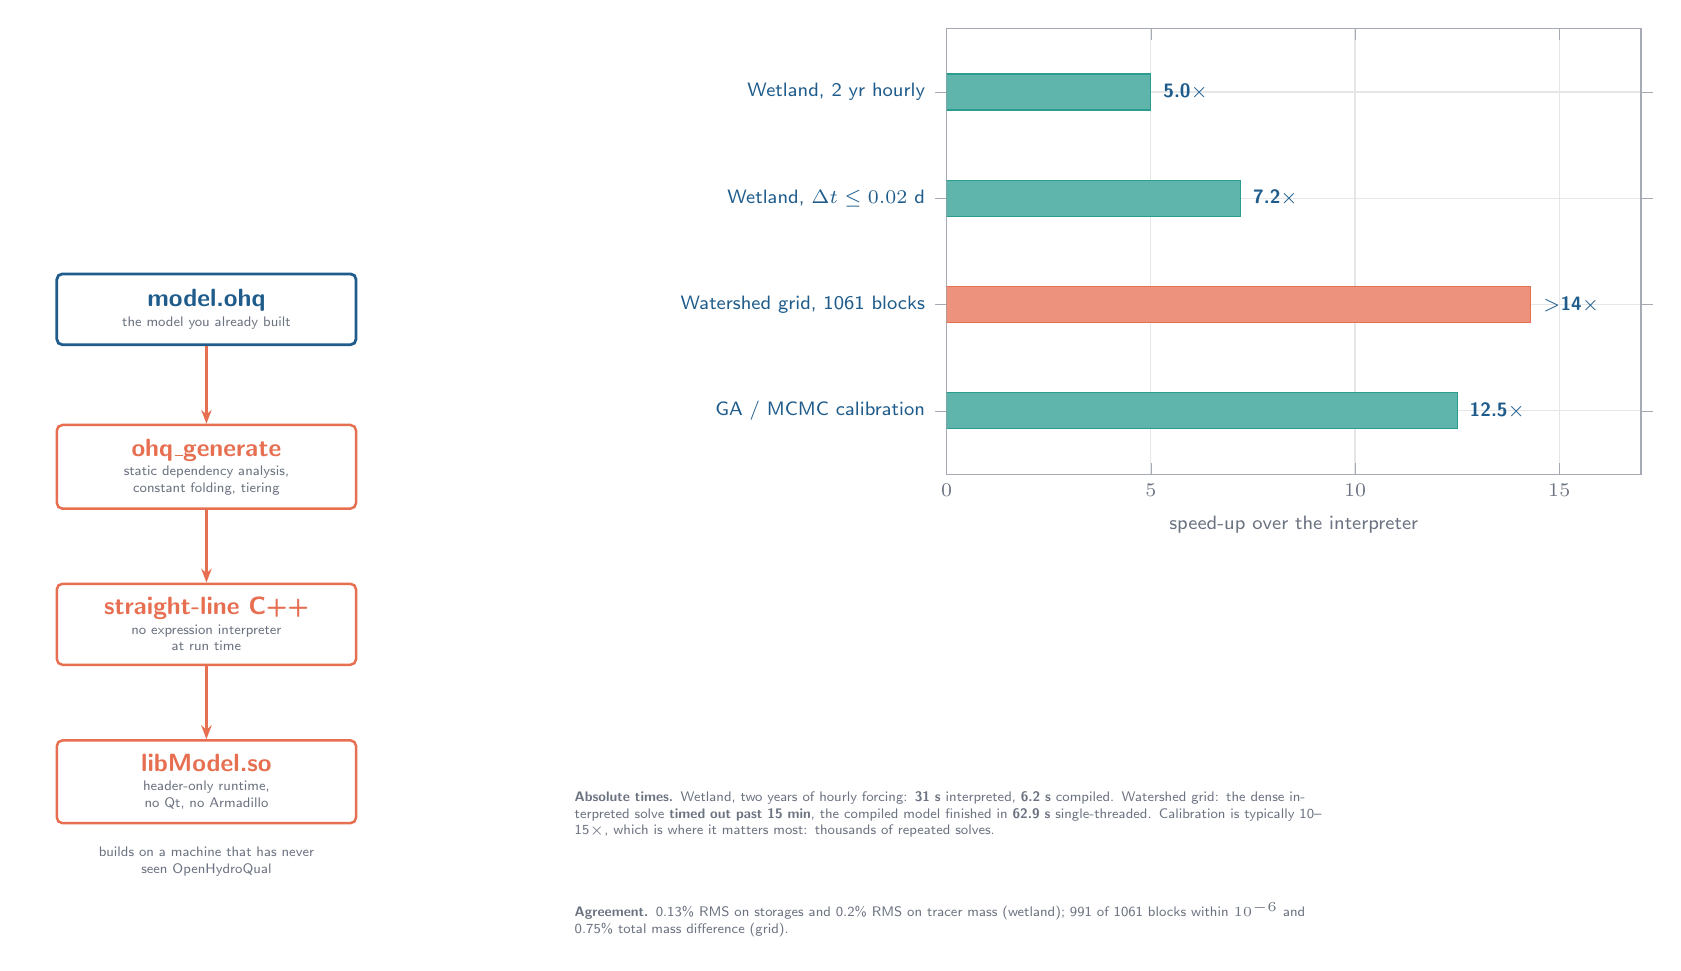
\begin{tikzpicture}[
  font=\sffamily,
  pstep/.style={draw=ohqrust, line width=0.9pt, fill=white, rounded corners=2pt, font=\tiny, text=ohqgrey,
               align=center, inner sep=5pt, minimum width=38mm, minimum height=9mm},
  psrc/.style={draw=ohqblue, line width=1pt, fill=white, rounded corners=2pt, font=\tiny, text=ohqgrey,
              align=center, inner sep=5pt, minimum width=38mm, minimum height=9mm},
  arr/.style={-{Stealth[length=5pt]}, ohqrust, line width=1pt},
  lbl/.style={font=\tiny, text=ohqgrey, align=center, inner sep=2pt},
]
\def\hd#1{\textbf{\color{ohqrust}\small #1}}
\def\hb#1{\textbf{\color{ohqblue}\small #1}}
\def\sb#1{\\[1pt]#1}

% ---------------- pipeline (left) -----------------------------------
\node[psrc]  (mdl) at (0, 3.0) {\hb{model.ohq}\sb{the model you already built}};
\node[pstep] (gen) at (0, 1.0) {\hd{ohq\_generate}\sb{static dependency analysis,\\constant folding, tiering}};
\node[pstep] (cpp) at (0,-1.0) {\hd{straight-line C++}\sb{no expression interpreter\\at run time}};
\node[pstep] (so)  at (0,-3.0) {\hd{libModel.so}\sb{header-only runtime,\\no Qt, no Armadillo}};

\draw[arr] (mdl) -- (gen);
\draw[arr] (gen) -- (cpp);
\draw[arr] (cpp) -- (so);

\node[lbl, anchor=north, text width=44mm] at ([shift={(0,-6pt)}]so.south)
  {builds on a machine that has never\\seen OpenHydroQual};

% ---------------- speed-ups (right) ---------------------------------
\begin{scope}[shift={(9.4,0.9)}]
\begin{axis}[
  width=10.4cm, height=7.2cm,
  xbar, xmin=0, xmax=17,
  bar width=13pt,
  y=13.5mm,
  symbolic y coords={cal,grid,wetdt,wet},
  ytick={cal,grid,wetdt,wet},
  yticklabels={%
    {GA / MCMC calibration},%
    {Watershed grid, 1061 blocks},%
    {Wetland, $\Delta t\le0.02$ d},%
    {Wetland, 2 yr hourly}},
  yticklabel style={font=\scriptsize, text=ohqblue},
  xlabel={speed-up over the interpreter},
  xlabel style={font=\scriptsize, text=ohqgrey},
  xtick={0,5,10,15},
  xticklabel style={font=\scriptsize, text=ohqgrey},
  axis line style={ohqgrey!60},
  tick style={ohqgrey!60},
  grid=major, major grid style={ohqgrey!18},
  enlarge y limits=0.20,
  nodes near coords style={font=\scriptsize\bfseries, text=ohqblue},
  every node near coord/.append style={anchor=west, xshift=1pt},
]
\addplot[fill=ohqteal!75, draw=ohqteal, bar shift=0pt,
         nodes near coords={12.5$\times$}] coordinates {(12.5,cal)};
\addplot[fill=ohqrust!75, draw=ohqrust, bar shift=0pt,
         nodes near coords={$>$14$\times$}] coordinates {(14.3,grid)};
\addplot[fill=ohqteal!75, draw=ohqteal, bar shift=0pt,
         nodes near coords={7.2$\times$}] coordinates {(7.2,wetdt)};
\addplot[fill=ohqteal!75, draw=ohqteal, bar shift=0pt,
         nodes near coords={5.0$\times$}] coordinates {(5.0,wet)};
\end{axis}
\end{scope}

\node[lbl, anchor=north west, text width=96mm, align=left]
  at (4.6,-3.05)
  {\textbf{Absolute times.} Wetland, two years of hourly forcing:
   \textbf{31 s} interpreted, \textbf{6.2 s} compiled. Watershed grid:
   the dense interpreted solve \textbf{timed out past 15 min}, the compiled
   model finished in \textbf{62.9 s} single-threaded. Calibration is typically
   10--15$\times$, which is where it matters most: thousands of repeated solves.};
\node[lbl, anchor=north west, text width=96mm, align=left]
  at (4.6,-4.45)
  {\textbf{Agreement.} 0.13\% RMS on storages and 0.2\% RMS on tracer mass
   (wetland); 991 of 1061 blocks within $10^{-6}$ and 0.75\% total mass
   difference (grid).};

\end{tikzpicture}
\end{document}
